\section{Introduction}
\label{sec:introduction}
\FloatBarrier % Now figures cannot float above section title
The main purpose of this experiment is to investigate the operation and characteristics of three different
types of flowmeter: venture meter, orifice plate meter and variable area meter in four different flowrates of 5, 10, 15, 20 L/min.
By researching the experimental data of these three flow meters at different water pressures, 
the energy loss of the water flowing through the meters was determined.
% Historical chart of CO2 emissions
%\begin{figure}[htb] % Here, top, bottom priority list
%   \centering
%  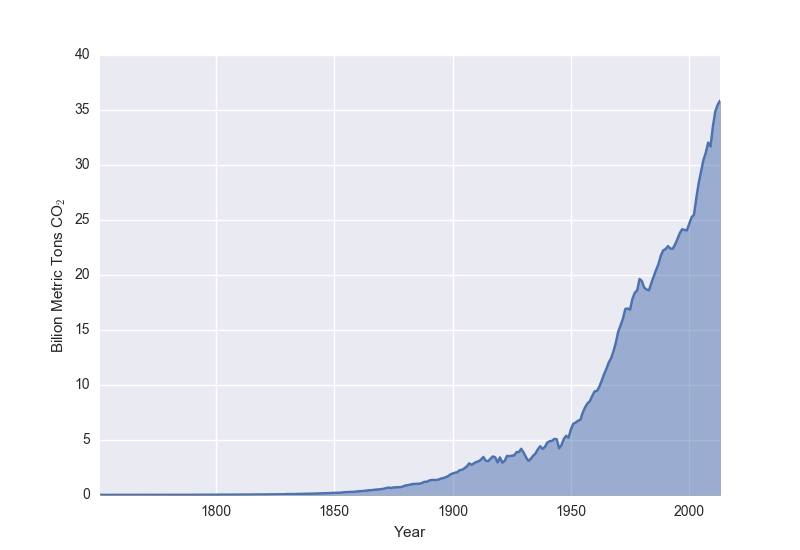
\includegraphics[scale=0.45]{Introduction/figures/Historic_CO2_Emission}
%    \caption{This text should be able to stand alone independent of text outside figure!}
%    \label{fig:intro_co2}
%\end{figure}